\documentclass[aspectratio=169]{beamer}
\usepackage[utf8]{luainputenc}
\usepackage{amssymb,amsmath}
\usepackage{graphicx}
\usepackage{tikz}
\usepackage{beamercolorthemetud}
\usepackage[backend=biber]{biblatex}
\usepackage{caption}
\captionsetup[figure]{font=scriptsize}

\usepackage{subcaption}
\usepackage[absolute,overlay]{textpos}
  \setlength{\TPHorizModule}{1mm}
  \setlength{\TPVertModule}{1mm}




\addbibresource{bibl.bib}
\setbeamertemplate{bibliography item}{\insertbiblabel}
\usepackage[english]{babel}
\usetheme[]{tud}
\setbeamercolor{background canvas}{bg=}
\setbeamerfont{frametitle}{size=\Large}
% Macros used by all lectures, but not necessarily by excercises

%%% General setup and dependencies:

% \usetheme[ddcfooter,nosectionnum]{tud}
%\usetheme[nosectionnum,pagenum,noheader]{tud}
\usetheme[]{tud}
% \usetheme[nosectionnum,pagenum]{tud}
\setbeamertemplate{enumerate items}[default]

% Increase body font size to a sane level:
\let\origframetitle\frametitle
% \renewcommand{\frametitle}[1]{\origframetitle{#1}\normalsize}
\renewcommand{\frametitle}[1]{\origframetitle{#1}\fontsize{10pt}{13.2}\selectfont}
\setbeamerfont{itemize/enumerate subbody}{size=\small} % tud defaults to scriptsize!
\setbeamerfont{itemize/enumerate subsubbody}{size=\small}
% \setbeamerfont{normal text}{size=\small}
% \setbeamerfont{itemize body}{size=\small}

\renewcommand{\emph}[1]{\textbf{#1}}

\def\arraystretch{1.3}% Make tables even less cramped vertically

\usepackage[english]{babel}
\usepackage[utf8]{inputenc}
\usepackage[T1]{fontenc}

%\usepackage{graphicx}
\usepackage[export]{adjustbox} % loads graphicx
\usepackage{import}
\usepackage{stmaryrd}
\usepackage[normalem]{ulem} % sout command
% \usepackage{times}
\usepackage{txfonts}
\usepackage{array}

% \usepackage[perpage]{footmisc} % reset footnote counter on each page -- fails with beamer (footnotes gone)
\usepackage{perpage}  % reset footnote counter on each page
\MakePerPage{footnote}

\usepackage{tikz}
\usetikzlibrary{arrows,positioning,decorations.pathreplacing}
% Inspired by http://www.texample.net/tikz/examples/hand-drawn-lines/
\usetikzlibrary{decorations.pathmorphing}
\pgfdeclaredecoration{penciline}{initial}{
    \state{initial}[width=+\pgfdecoratedinputsegmentremainingdistance,
    auto corner on length=1mm,]{
        \pgfpathcurveto%
        {% From
            \pgfqpoint{\pgfdecoratedinputsegmentremainingdistance}
                      {\pgfdecorationsegmentamplitude}
        }
        {%  Control 1
        \pgfmathrand
        \pgfpointadd{\pgfqpoint{\pgfdecoratedinputsegmentremainingdistance}{0pt}}
                    {\pgfqpoint{-\pgfdecorationsegmentaspect
                     \pgfdecoratedinputsegmentremainingdistance}%
                               {\pgfmathresult\pgfdecorationsegmentamplitude}
                    }
        }
        {%TO 
        \pgfpointadd{\pgfpointdecoratedinputsegmentlast}{\pgfpoint{1pt}{1pt}}
        }
    }
    \state{final}{}
}
\tikzset{handdrawn/.style={decorate,decoration=penciline}}
\tikzset{every shadow/.style={fill=none,shadow xshift=0pt,shadow yshift=0pt}}
% \tikzset{module/.append style={top color=\col,bottom color=\col}}

% Use to make Tikz attributes with Beamer overlays
% http://tex.stackexchange.com/a/6155
\tikzset{onslide/.code args={<#1>#2}{%
  \only<#1| handout:0>{\pgfkeysalso{#2}} 
}}
\tikzset{onslideprint/.code args={<#1>#2}{%
  \only<#1>{\pgfkeysalso{#2}} 
}}

%%% Title -- always set this first

\newcommand{\defineTitle}[3]{
	\newcommand{\lectureindex}{#1}
	\title{Formale Systeme}
	\subtitle{\href{\lectureurl}{#1. Vorlesung: #2}}
	\author{\href{https://iccl.inf.tu-dresden.de/web/Markus_Kr\%C3\%B6tzsch}{Markus Kr\"{o}tzsch}\\[1ex]Professur für Wissensbasierte Systeme}
	\date{#3}
	\datecity{TU Dresden}
% 	\institute{CC-By 3.0, sofern keine anderslautenden Bildrechte angegeben sind}
}

%%% Table of contents:

\RequirePackage{ifthen}

\newcommand{\highlight}[2]{%
	\ifthenelse{\equal{#1}{\lectureindex}}{\alert{#2}}{#2}%
}

\def\myspace{-0.7ex}
\newcommand{\printtoc}{
\begin{tabular}{r@{$\quad$}l}
\highlight{1}{1.} & \highlight{1}{Willkommen/Einleitung formale Sprachen}\\[\myspace]
\highlight{2}{2.} & \highlight{2}{Grammatiken und die Chomsky-Hierarchie}\\[\myspace]
\highlight{3}{3.} & \highlight{3}{Endliche Automaten}\\[\myspace]
\highlight{4}{4.} & \highlight{4}{Complexity of FO query answering}\\[\myspace]
\highlight{5}{5.} & \highlight{5}{Conjunctive queries}\\[\myspace]
\highlight{6}{6.} & \highlight{6}{Tree-like conjunctive queries}\\[\myspace]
\highlight{7}{7.} & \highlight{7}{Query optimisation}\\[\myspace]
\highlight{8}{8.} & \highlight{8}{Conjunctive Query Optimisation / First-Order~Expressiveness}\\[\myspace]
\highlight{9}{9.} & \highlight{9}{First-Order~Expressiveness / Introduction to Datalog}\\[\myspace]
\highlight{10}{10.} & \highlight{10}{Expressive Power and Complexity of Datalog}\\[\myspace]
\highlight{11}{11.} & \highlight{11}{Optimisation and Evaluation of Datalog}\\[\myspace]
\highlight{12}{12.} & \highlight{12}{Evaluation of Datalog (2)}\\[\myspace]
\highlight{13}{13.} & \highlight{13}{Graph Databases and Path Queries}\\[\myspace]
\highlight{14}{14.} & \highlight{14}{Outlook: database theory in practice}
\end{tabular}
}

\newcommand{\overviewslide}{%
\begin{frame}\frametitle{Overview}
\printtoc
\medskip

Siehe \href{\lectureurl}{course homepage [$\Rightarrow$ link]} for more information and materials
\end{frame}
}

%%% Colours:
\usepackage{xcolor,colortbl}
\definecolor{redhighlights}{HTML}{FFAA66}
\definecolor{lightblue}{HTML}{55AAFF}
\definecolor{lightred}{HTML}{FF5522}
\definecolor{lightpurple}{HTML}{DD77BB}
\definecolor{lightgreen}{HTML}{55FF55}
\definecolor{darkred}{HTML}{CC4411}
\definecolor{darkblue}{HTML}{176FC0}%{1133AA}
\definecolor{nightblue}{HTML}{2010A0}%{1133AA}
\definecolor{alert}{HTML}{176FC0}
\definecolor{darkgreen}{HTML}{36AB14}
\definecolor{strongyellow}{HTML}{FFE219}
\definecolor{devilscss}{HTML}{666666}

\newcommand{\redalert}[1]{\textcolor{darkred}{#1}}

%%% Style commands

\newcommand{\quoted}[1]{\texttt{"}{#1}\texttt{"}}
\newcommand{\squote}{\texttt{"}} % straight quote
\newcommand{\Sterm}[1]{\ensuremath{\mathtt{\textcolor{purple}{#1}}}}    % letters in alphabets
\newcommand{\Snterm}[1]{\textsf{\textcolor{darkblue}{#1}}} % nonterminal symbols
\newcommand{\Sntermsub}[2]{\ensuremath{\Snterm{#1}_{\Snterm{#2}}}} % nonterminal symbols
\newcommand{\Slang}[1]{\textbf{\textcolor{black}{#1}}}    % languages
\newcommand{\Slangsub}[2]{\ensuremath{\Slang{#1}_{\Slang{#2}}}}    % languages
% Code
\newcommand{\Scode}[1]{\textbf{#1}}    % reserved words in program listings, e.g., "if"
\newcommand{\Scodelit}[1]{\textcolor{purple}{#1}}    % literals in program listings, e.g., strings
\newcommand{\Scomment}[1]{\textcolor{gray}{#1}}    % comment in program listings

\newcommand{\epstrastar}{\mathrel{\mathord{\stackrel{\epsilon}{\to}}{}^*}} % transitive reflexive closure of epsilon transitions in an epslion-NFA

\newcommand{\narrowcentering}[1]{\mbox{}\hfill#1\hfill\mbox{}}

\newcommand{\Smach}[1]{\ensuremath{\mathcal{#1}}}    % machines

\newcommand{\mytrue}{\Scodelit{1}}
\newcommand{\myfalse}{\Scodelit{0}}
% \newcommand{\emptyClause}{\bot}

\newcommand{\Scomplclass}[1]{{\textsc{#1}}} % font for complexity classes, used on slides where the "too many alphabets" LaTeX error appears when using the correct sc font :-(
% \newcommand{\complclass}[1]{\ensuremath{\mathsc{#1}}} % font for complexity classes

%%% Slide layout commands:

\newcommand{\sectionSlide}[1]{
\frame{\begin{center}
\LARGE
#1
\end{center}}
}
\newcommand{\sectionSlideNoHandout}[1]{
\frame<handout:0>{\begin{center}
\LARGE
#1
\end{center}}
}

\newcommand{\mydualbox}[3]{%
 \begin{minipage}[t]{#1}
 \begin{beamerboxesrounded}[upper=block title,lower=block body,shadow=true]%
    {\centering\usebeamerfont*{block title}#2}%
    \raggedright%
    \usebeamerfont{block body}
%     \small
    #3%
  \end{beamerboxesrounded}
  \end{minipage}
}
% 
\newcommand{\myheaderbox}[2]{%
 \begin{minipage}[t]{#1}
 \begin{beamerboxesrounded}[upper=block title,lower=block title,shadow=true]%
    {\centering\usebeamerfont*{block title}\rule{0pt}{2.6ex} #2}%
  \end{beamerboxesrounded}
  \end{minipage}
}

\newcommand{\mycontentbox}[2]{%
 \begin{minipage}[t]{#1}%
 \begin{beamerboxesrounded}[upper=block body,lower=block body,shadow=true]%
    {\centering\usebeamerfont*{block body}\rule{0pt}{2.6ex}#2}%
  \end{beamerboxesrounded}
  \end{minipage}
}

\newcommand{\mylcontentbox}[2]{%
 \begin{minipage}[t]{#1}%
 \begin{beamerboxesrounded}[upper=block body,lower=block body,shadow=true]%
    {\flushleft\usebeamerfont*{block body}\rule{0pt}{2.6ex}#2}%
  \end{beamerboxesrounded}
  \end{minipage}
}

% label=180:{\rotatebox{90}{{\footnotesize\textcolor{darkgreen}{Beispiel}}}}
% \hspace{-8mm}\ghost{\raisebox{-7mm}{\rotatebox{90}{{\footnotesize\textcolor{darkgreen}{Beispiel}}}}}\hspace{8mm}
\newcommand{\examplebox}[1]{%
	\begin{tikzpicture}[decoration=penciline, decorate]
		\pgfmathsetseed{1235}
		\node (n1) [decorate,draw=darkgreen, fill=darkgreen!10,thick,align=left,text width=\linewidth, inner ysep=2mm, inner xsep=2mm] at (0,0) {#1};
% 		\node (n2) [align=left,text width=\linewidth,inner sep=0mm] at (n1.92) {{\footnotesize\raisebox{3mm}{\textcolor{darkgreen}{Beispiel}}}};
% 		\node (n2) [decorate,draw=darkgreen, fill=darkgreen!10,thick, align=left,text width=\linewidth,inner sep=2mm] at (n1.90) {{\footnotesize\raisebox{0mm}{\textcolor{darkgreen}{Beispiel}}}};
	\end{tikzpicture}%
}%

\newcommand{\codebox}[1]{%
	\begin{tikzpicture}[decoration=penciline, decorate]
		\pgfmathsetseed{1236}
		\node (n1) [decorate,draw=strongyellow, fill=strongyellow!10,thick,align=left,text width=\linewidth, inner ysep=2mm, inner xsep=2mm] at (0,0) {#1};
	\end{tikzpicture}%
}%

\newcommand{\defbox}[1]{%
	\begin{tikzpicture}[decoration=penciline, decorate]
		\pgfmathsetseed{1237}
		\node (n1) [decorate,draw=darkred, fill=darkred!10,thick,align=left,text width=\linewidth, inner ysep=2mm, inner xsep=2mm] at (0,0) {#1};
	\end{tikzpicture}%
}%

\newcommand{\theobox}[1]{%
	\begin{tikzpicture}[decoration=penciline, decorate]
		\pgfmathsetseed{1240}
		\node (n1) [decorate,draw=darkblue, fill=darkblue!10,thick,align=left,text width=\linewidth, inner ysep=2mm, inner xsep=2mm] at (0,0) {#1};
	\end{tikzpicture}%
}%

\newcommand{\anybox}[2]{%
	\begin{tikzpicture}[decoration=penciline, decorate]
		\pgfmathsetseed{1240}
		\node (n1) [decorate,draw=#1, fill=#1!10,thick,align=left,text width=\linewidth, inner ysep=2mm, inner xsep=2mm] at (0,0) {#2};
	\end{tikzpicture}%
}%


\newsavebox{\mybox}%
\newcommand{\doodlebox}[2]{%
\sbox{\mybox}{#2}%
	\begin{tikzpicture}[decoration=penciline, decorate]
		\pgfmathsetseed{1238}
		\node (n1) [decorate,draw=#1, fill=#1!10,thick,align=left,inner sep=1mm] at (0,0) {\usebox{\mybox}};
	\end{tikzpicture}%
}%
\newcommand{\widedoodlebox}[2]{%
\sbox{\mybox}{#2}%
	\begin{tikzpicture}[decoration=penciline, decorate]
		\pgfmathsetseed{1238}
		\node (n1) [decorate,draw=#1, fill=#1!10,thick,align=left,inner sep=1mm,text width=\linewidth] at (0,0) {\usebox{\mybox}};
	\end{tikzpicture}%
}%



\title{App Idea Presentation: MeetForSport}
\author{Mattis Lahr, Felix Fischer}
\date{19.11.2021}

\einrichtung{\hspace{-1pt}Institute of Systems Architecture}
\datecity{Dresden}




\AtBeginSection[]{\partpage{\usebeamertemplate***{part page}}}
\begin{document}
\maketitle



\begin{frame}
    \frametitle{Table of Contents}
    \tableofcontents
\end{frame}





\section{Scenario}
\begin{frame}   
\frametitle{Our Scenario}
Imagine:
    \begin{itemize}	
	 	\item You are an active person
	 	\item You like to play team sports but don’t know how to find enough other people interested in the sport of your choice to actually built big enough teams OR
	 	\item You just want to find other people who are interested in the same sports as you to do them together
    \end{itemize}
\end{frame}


%\section{Problem}
%\begin{frame}   
%	While there are many (fitness) Apps out on the market, none really
%	addresses the problem of lacking people to play with. Joining an active
%	community is still part of ones social circle, whereas every other aspect of
%	our live can be enhanced by multimedia devices.
%	\end{frame}


\section{Our Idea}
\begin{frame}   
\frametitle{What is our idea?}
Our Solution is rather simple and draws its inspiration from other networking apps.
Our App would try to solve these problems. It is supposed to become an App that
    \begin{itemize}	
		\item enables you to find people interested in the same sport
	 	\item suggests places for your activity 
	 	\item lets you set up meeting times and points
	 	\item builds a community around your activities 
    \end{itemize}
\end{frame}

\begin{frame}   
\frametitle{Target Group}
The App will target persons of nearly all ages who are interested in physical group activities and who are open to meet new people. 
\end{frame}

\begin{frame}   
	\frametitle{Personas}{\textbf{Fred Flintstone Part 1:}}

	This is Fred Flintstone. He is 23 years old and studies Physics in his 7th semester. 
He's from Dresden and currently resids in the studentdorm. 
When not studying, he takes up his old hobby of playing football, that he started in preschool. If the weather is bad, he fires up his playstation to join his friends in some multiplayer game.
On his weekends, Fred likes to meet up with people in pubs or clubs.

However, one thing really annoys him... unreliable friends. Setting up sport events with them proves difficult in many ways.
One of them will surely have forgotten the date, one of them cancels last second and others allways run late.
So while he enjoys playing football, setting up the event is quite a challenge.
\end{frame}

\begin{frame}   
	\frametitle{Personas}{\textbf{Fred Flintstone Part 2:}}

\begin{itemize}
	\item personal information:
	\begin{itemize}
		\item Age: 23
		\item Profession: physics stundent (7th semester)
		\item Living condition: alone, stundentdorm
		\item Interests: football, meeting friends, playing (computer) games, parties
		\item personal trades: emphatic, organized, spontaneous, tech-savvy
\end{itemize}
\end{itemize}

\end{frame}

\begin{frame}   
	\frametitle{Personas}{\textbf{Martina Ödegaard Part 1:}}

	This is Martina Ödegaard. She is a 36 year old car mechanic. She is originally from Frankfurt(Oder) where she also learned her profession. She moved to Dresden 12 years ago, after moving in with her partner, who was already living there. 
\end{frame}

\begin{frame}   
	\frametitle{Personas}{\textbf{Martina Ödegaard Part 2:}}

\begin{itemize}
	\item personal information:
	\begin{itemize}
		\item Age: 36
		\item Profession: car mechanic
		\item Living condition: married, living in an appartment with her partner (37) and her two kids (5 and 8)
		\item Interests: reading, running, meeting with friends
		\item personal trades:
	\end{itemize}

\end{itemize}

\end{frame}

\section{Key Features}

\begin{frame}
\frametitle{\centerline{Creating a new activity}}
\begin{figure}
	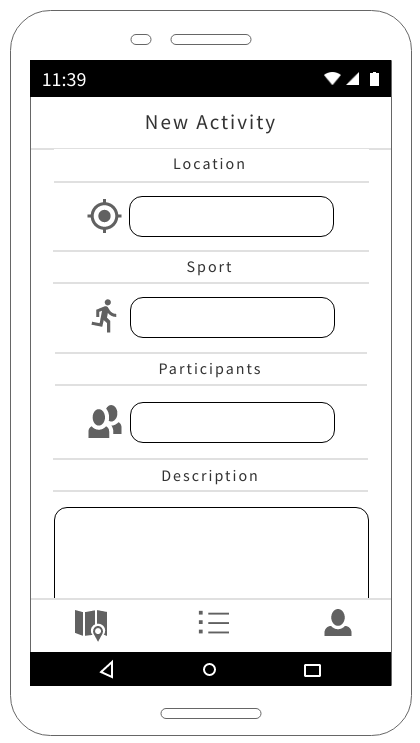
\includegraphics[width=0.25\textwidth]{media/new_activity.png}
\end{figure}
\end{frame}

\begin{frame}
\frametitle{\centerline{A list of upcoming activities with filter options}}
\begin{figure}
	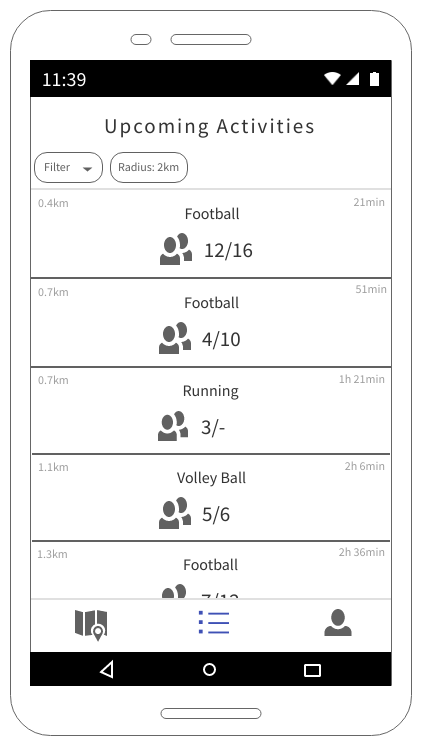
\includegraphics[width=0.25\textwidth]{media/upcoming_activities.png}
\end{figure}
\end{frame}


\begin{frame}
\frametitle{\centerline{An interactive map that displays activities}}
\begin{figure}
	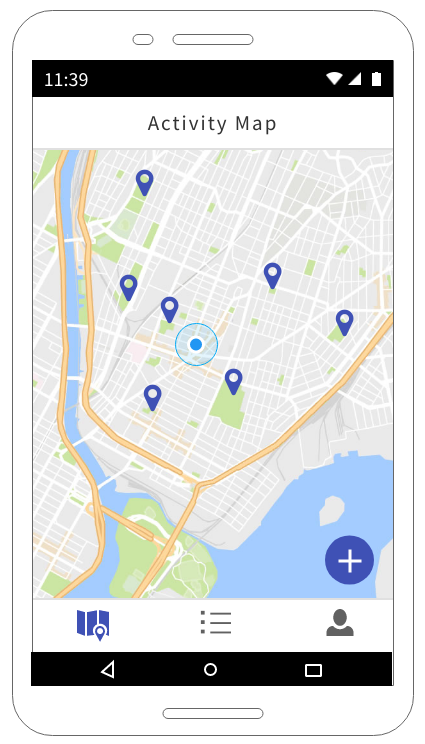
\includegraphics[width=0.25\textwidth]{media/activity_map.png}
\end{figure}
\end{frame}


\begin{frame}
\frametitle{\centerline{A customizable user profile}}
\begin{figure}
	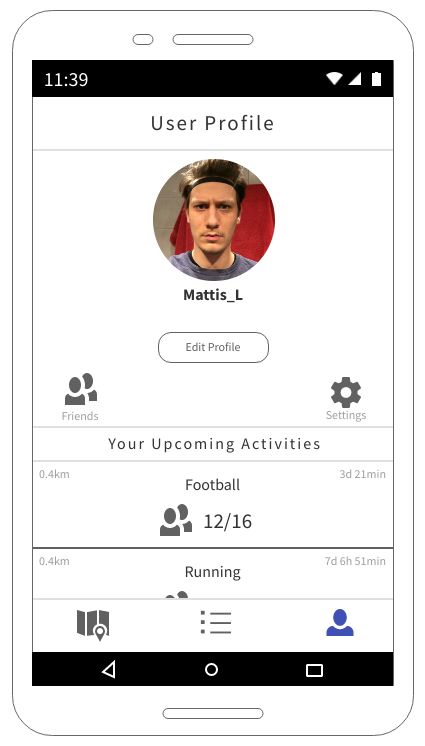
\includegraphics[width=0.25\textwidth]{media/user_profile.png}
\end{figure}
\end{frame}




\section{Challenges}
\begin{frame}
	\begin{itemize}
		\item build/find an efficient way to find locations
		\item assign each sport a set of requirements (e.g. important features the location needs)
		\item build a user database
		\item build an organizer 
		\item implement interaction possibilities
	\end{itemize}
\end{frame}

\end{document}